\chapter{SynVisio}

Our most significant contribution in this research was the development of SynVisio, an online platform to explore syteny by mapping syntenic blocks that are highly conserved and long enough to be significant between a given pair of genomes or within a single genome. In this chapter, we first discuss the different modes SynVisio offers for synteny analysis and how each one operates. We then explore the various features SynVisio provides to enhance user experience with the tool. Finally, we discuss the software implementation of the tool and then elaborate on the choices made in the web architecture of the system.

\section{System Overview}
SynVisio is a multi scale genome browser that can be accessed through the web to explore genomic conservation. It lets researchers upload output files of a synteny detection system of their choice and generates visualizations on-demand from the information in these files. It offers two analysis modes: Single Level and Multi-Level. In the first mode, users can compare genomes two at a time through a dashboard where synteny is visualized as both a dot plot and a linked parallel plot. The charts are accompanied by a filter panel where the conserved genomic blocks can be filtered based on features such as the degree of similarity. In the second mode, researchers can compare several genomes at a time through multi-level representations such as hive plots and stacked parallel plots. To aid researchers in their visual exploration of synteny, SynVisio lets them annotate the generated charts with additional tracks in the form of histograms, heat-maps and other basic plots. Additional features are also provided, such as a gene search panel to look for specific genes by gene ID and the ability to export generated charts for publication.


\section{Analysis Mode}
Gene sequences can be compared in different ways, depending on the underlying biological question. This means syteny analysis can vary between visualizing simple pairwise matches between two genomes to performing  multi-way comparisons across several genomes at once. The availability of datasets and their inherent quality also plays into the kind of analysis that can be done. Whole-genome alignment, for example is usually done pairwise as looking for matches can be faster when the subset of available matches is low. Additionally, in the context of synteny detection, which is anchor-based, identifying common markers between multiple genomes is difficult\cite{wang2012mcscanx}. However when the data is available, multi-way comparisons can offer better insights and tackle more significant questions like pan-genome synteny. Thus SynVisio offers both a Single and a Multi Level analysis mode depending on the researchers choice and the availability of data.

\subsection{Single Level Analysis}
This is default mode in which SynVisio operates and is meant for exploratory tasks as it presents the collinearity between a selected set of chromosomes in two different visual representations and lets users filter the collinear blocks on the fly. Although our system operates as a dashboard with multiple representations in coordinated views, we also offer users the ability to look only at one particular representation through the configuration page. This is meant to make our system unopinionated in the choice of visual representation and let users decide on how they want their data to be visualized. 

\begin{figure}
  \centering
  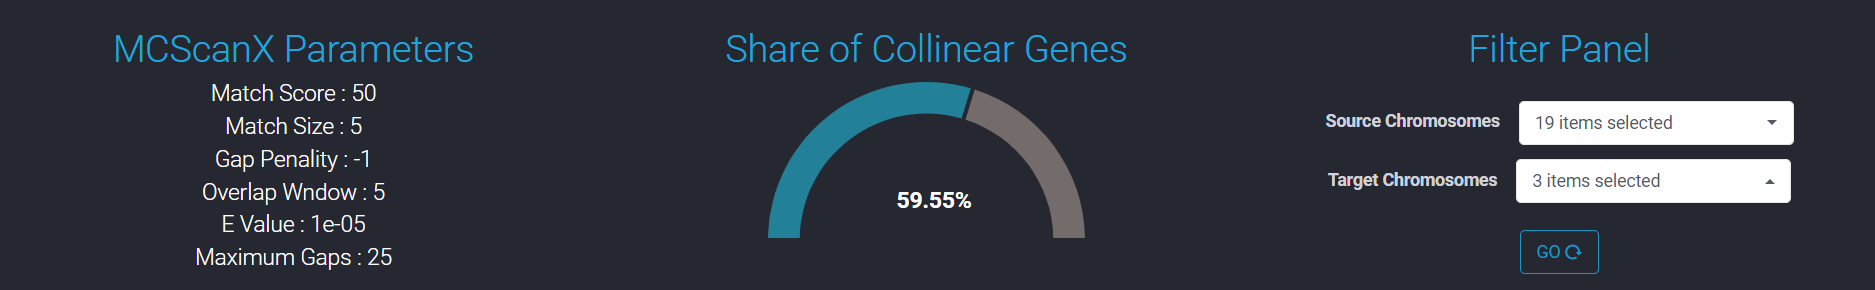
\includegraphics[width=1\linewidth]{images/ch_5_baseparameters.PNG}
  \captionof{figure}{Synteny detection parameters and level of collinearity presented along with toggles to select source and target chromosomes.}
  \label{fig:ch_5_baseparameters}
\end{figure}


The first step involved in using the dashboard is providing an input dataset, for this, users can either upload their own datasets or use existing sample files. We have already processed several datasets depicting genome conservation on a wide range of species. These are available on the homepage of our application and are updated on a regular basis.Some of the examples include self synteny in \textit{Brassica napus}(canola), cross synteny between \textit{Oriza sativa} (rice) and \textit{Sorghum bicolor}(broom-corn) and cross synteny between \textit{Arabidopsis thaliana}(thale cress) and \textit{Vitis vinifera}(grapevine). After the initial data uploading and processing stage is complete, basic information about the parameters used in the synteny detection process is presented along with the percentage share of collinearity present in the files accompanied with toggles to select the source and target chromosomes as shown in Figure \ref{fig:ch_5_baseparameters}. If outputs of synteny detection systems other than MCScanX are uploaded the parameters tab and the percentage share of collinear genes chart are replaced with a textual panel describing the features of the data on file including a list of all unique chromosomes and the total number of collinear blocks. The list of chromosomes is ordered alpha-numerically to divide the different species into distinct groups and make it easier to pick chromosomes sequentially. Additional buttons are also provided to either \textit{Select All} or \textit{Clear All} options in both the drop-drown lists intended for choosing chromosomes. The dashboard operates in three views based on the level of genomic resolution, and each of these stages are described individually below.

\begin{figure}
  \centering
  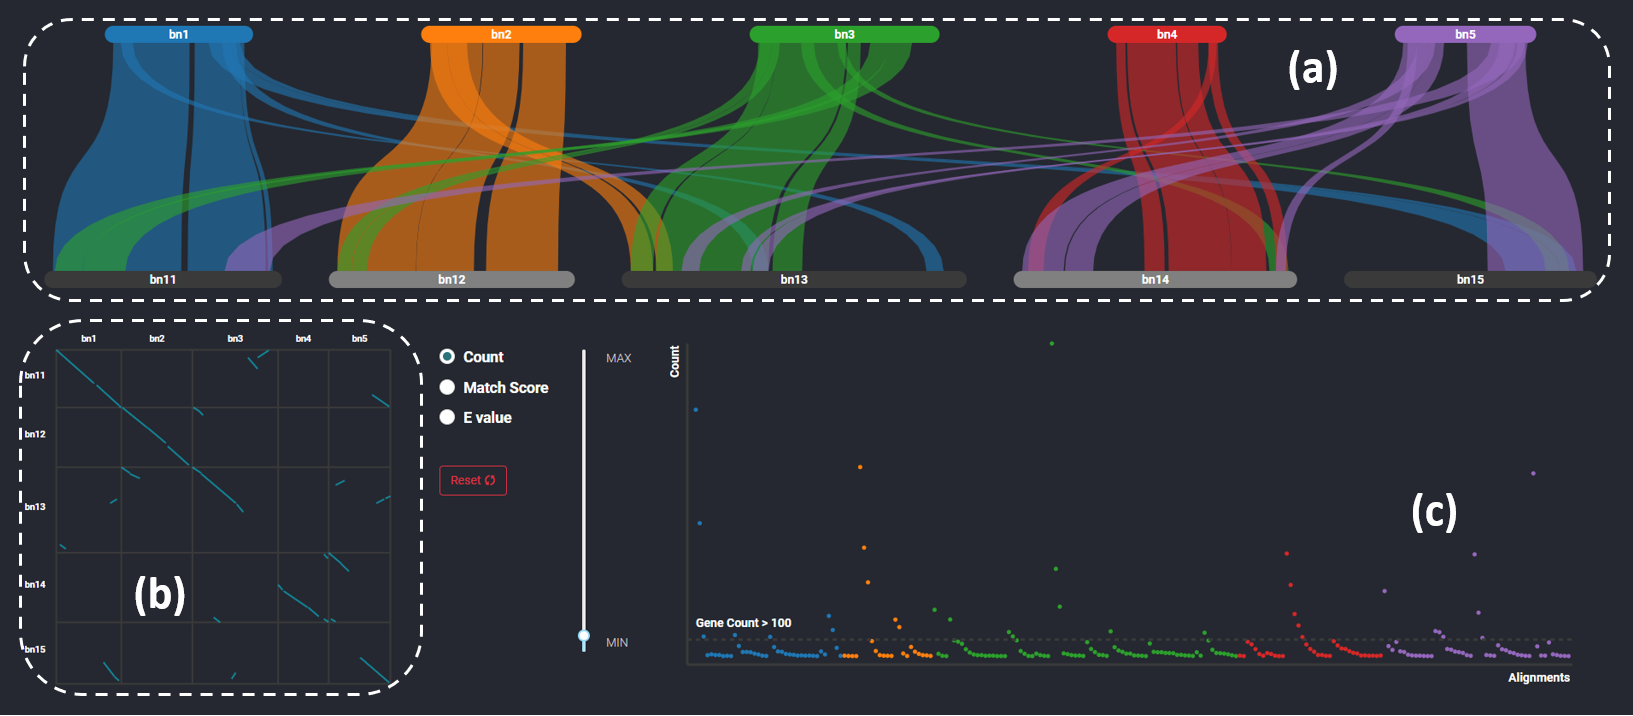
\includegraphics[width=1\linewidth]{images/ch_1_dashboard.PNG}
  \captionof{figure}{Genome View in the Single Analysis Mode with the following components: \textbf{a)} Parallel Link Plot \textbf{b)}Dot plot and \textbf{c)} Filter panel}
  \label{fig:ch_4_dashboard}
\end{figure} 

\textit{Genome View:}
This view is chosen by default when a user selects more than one chromosome in the source or target selection drop-down and is intended for observing large scale patterns at the genome level.
The first visualization presented at the top is a parallel link plot where syntenic collinear blocks are connected by coloured ribbons, as shown in Figure \ref{fig:ch_4_dashboard}. The source chromosomes are laid out on the top and the target chromosomes are spread out at the bottom. The size of the chromosomes are calculated based on the genomic sizes of the chromosomes and the available screen width to ensure that the visualizations are responsive across different screen sizes. Chromosomes in the source layer are coloured using a chromatic 10 point color scale derived from ColorBrewer\cite{colorbrewer} and are set to repeat after every 10 chromosomes as humans cannot perceive differences beyond a dozen colours\cite{ware2012information}.The connecting ribbons represent collinear blocks with the colour of a ribbon representing its source chromosome. These ribbons can have varying widths at either end due to the size of the collinear block they represent. Although collinear blocks have the same gene count at either side, the width of the block in terms of base pairs can be quite different at either side due to variable gap sizes between individual genes. This scaled representation of connected ribbons can also mean that certain ribbons can end up being smaller than a single pixel in width due to their small genomic size. So we clamp our scale at the lower end to 2 pixels to ensure that extremely small ribbons are still represented as 2 pixel wide lines instead of ribbons.


\begin{figure}
  \centering
  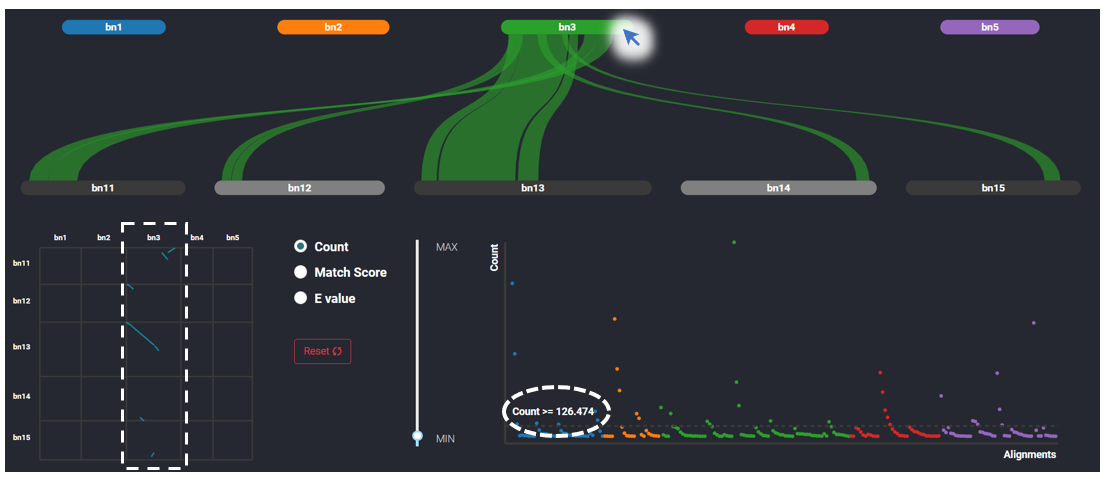
\includegraphics[width=1\linewidth]{images/ch_5_genome_view_2.PNG}
  \captionof{figure}{Genome View in the Single Analysis Mode with \textit{Chromosome 3} selected demonstrating the coordinated action being replicated in the Dot plot and the filter panel active with a target gene count set using the slider. } 
  \label{fig:ch_5_genome_view_2}
\end{figure} 


While the parallel link chart is designed to take half of the available vertical space, the other half is made up of a dot plot and an adaptive filter panel consisting of a scatter plot. The dot plot, as explained in the visual design chapter, uses positional encoding and represents collinear blocks as either dots or lines in a 2-dimensional matrix. To ensure that tiny collinear blocks are still represented on the screen, we limit them to single pixel wide dots on the chart while larger conserved blocks are encoded as lines. The dot plot works in a coordinated manner with the parallel link plot, and so any action in one is also reflected in the other, as shown in figure \ref{fig:ch_5_genome_view_2}. Since the dot plot is always meant to be square, it has a fixed aspect ratio, and thus the filter panel expands to fill the remaining horizontal space. It provides filtering through three parameters: Gene count, Match Score, and E(expect) value. It is set to filter using gene count by default but can be changed using the radio buttons provided to the left. To offer users context into the parameter being filtered, its values across all the collinear gene blocks are visualized as a simple scatter plot. Every collinear gene block is represented by a single dot irrespective of its size and is colour coded to correspond to the source chromosomes in the parallel plot. The scale of the scatter plot is adaptive and automatically changes based on the parameter in question. Gene count and Match Score correspond to the number of genes in a collinear block and the alignment score assigned to that block, respectively, and are represented in a linear scale. E-value or expect value is the measure of the probability that a match has occurred by chance, and owing to the wide range in which this value can be reported it is represented in a logarithmic scale. Researchers can use the slider to control the visibility of collinear blocks they see in the other two views. The position of the slider on the chart is represented with a dashed line that is annotated with the value at which the charts are currently being filtered as shown in figure \ref{fig:ch_5_genome_view_2}.


\begin{figure}[h]
  \centering
  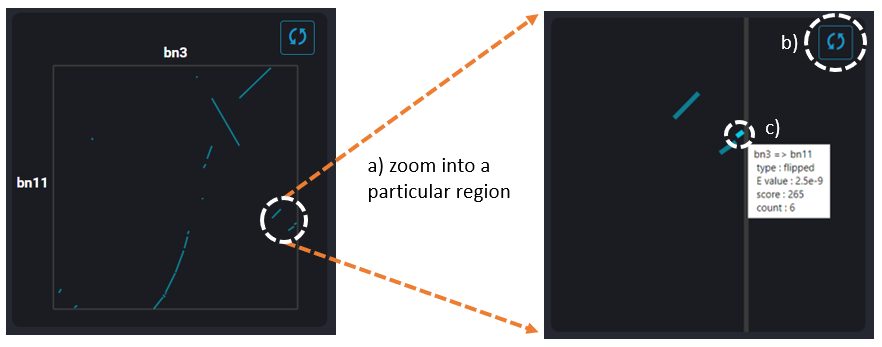
\includegraphics[width=.95\linewidth]{images/ch_5_chromosome_view.PNG}
  \captionof{figure}{Dot plot in the Chromosome View showing the ability to zoom into a particular region of interest (a), reset the zoom to the original state (b) and view additional information about a conserved block (c).} 
  \label{fig:ch_5_chromosome_view}
\end{figure} 

\textit{Chromosome View:} This view can be triggered in two ways, either by selecting a single source and a target chromosome using the drop-down selectors, or by clicking on a source and a target chromosome in the genome view. This acts as the logical second stage in exploring a genome where researchers can focus on a particular pair of chromosomes. At this stage, the layout of the visual representations remains the same however the visual encoding of colours to identify chromosomes is replaced with the orientation of the conserved regions with forward matched conserved regions represented as blue ribbons and reverse matched conserved regions represented in red. The adaptive filter panel also functions in the same way as in the genome view, but the dots in the scatter plot are not colour coded anymore to represent their chromosomal source. In this stage users are allowed to explore small scale patterns in conservation and thus have the ability to zoom into a particular part of the chart using mouse-based interactions, as shown in figure \ref{fig:ch_5_chromosome_view}. This feature is available to both the parallel plot and the dot plot, and the charts are provided with a reset button to readjust the scale of the charts to their original state. Finally, hovering the mouse over a conserved region in either plot will let users see additional information about that gene-block in an on-screen tool-tip.



\begin{figure}[h]
  \centering
  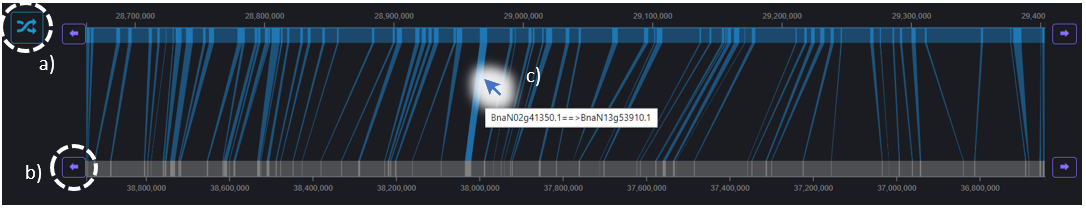
\includegraphics[width=1\linewidth]{images/ch_5_block_view.PNG}
  \captionof{figure}{Visualization in the Gene-Block View: a) Toggle button to flip the target gene block when exploring reverse matched gene blocks. b) Buttons to move the tracks horizontally along any one direction. c) On-screen tool-tip invoked by a mouse hover showing the source and target \textit{gene IDs} for a particular gene link.} 
  \label{fig:ch_5_block_view}
\end{figure} 

\textit{Gene-Block View:} This is the final view in the exploratory dashboard and can only be accessed from the chromosome view by double-clicking on a particular gene block in either of the two plots that are available at that level. It offers an in-depth view of each of the constituent genes in a collinear gene block and only has a single parallel plot representation. Every connected link represents a single gene and the size of the link is based on the number of base pairs in that gene. This plot can be zoomed in just like the plots in the chromosome view, however, the zoom is applied to the horizontal scale, which means after zooming in at a point, users can then pan the chart either to the left or right look at adjacent genes. Users can zoom in to a large cluster of genes to look at every single gene pair and get their \textit{gene IDs} by hovering over a connected link. The horizontal zoom however, can cause distortion when linked genes are far apart, causing them to stretch when zoomed in. To address this issue, we provided the tracks with two buttons on either side of both the source and target tracks. These can be used to shift the scale in the required direction to ensure that the gene pairs under investigation are not distorted and instead correctly lined up. Another common issue that can occur in this view is the visual occlusion problem due to a high number of crossing in an inverted gene block. Gene pairs in an inverted gene block are linked across the opposite ends of the gene block and so any zooming into the gene block at this stage would cause the genes to stretch further apart. To address this issue, we provide a toggle button next to the chart whenever a gene block is identified to be a reverse matched conserved region. This button selectively flips the target(bottom) genome scale alone, causing the gene pairs to line without any crossings, as shown in figure \ref{fig:ch_5_block_view_invert}. 

\begin{figure}
  \centering
  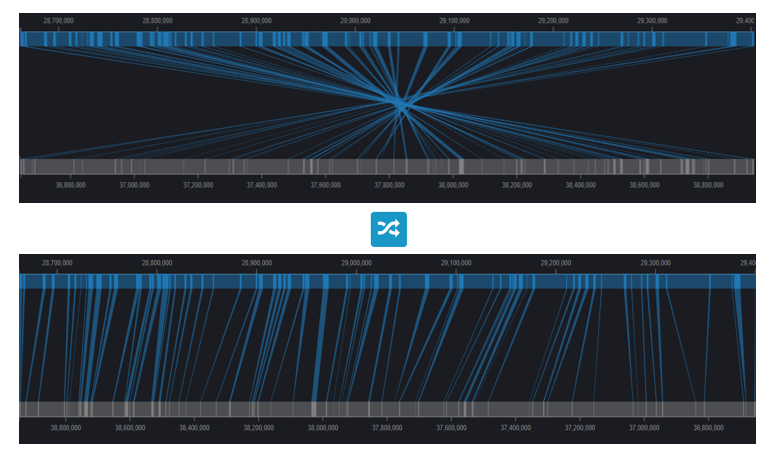
\includegraphics[width=1\linewidth]{images/ch_5_block_view_invert.PNG}
  \captionof{figure}{Conserved regions that have undergone reversals(top) can be flipped along the target genome using the toggle button to provide an uncluttered representation(bottom). } 
  \label{fig:ch_5_block_view_invert}
\end{figure} 

\subsection{Multi Level Analysis}
This mode can be enable by selecting the \textit{Multi-Level Analysis} radio button under plot characteristics in the configuration tab of SynVisio and there are 2 basic kinds of visualizations that are offered in this mode : Tree plot and a Hive plot.

\begin{figure}
  \centering
  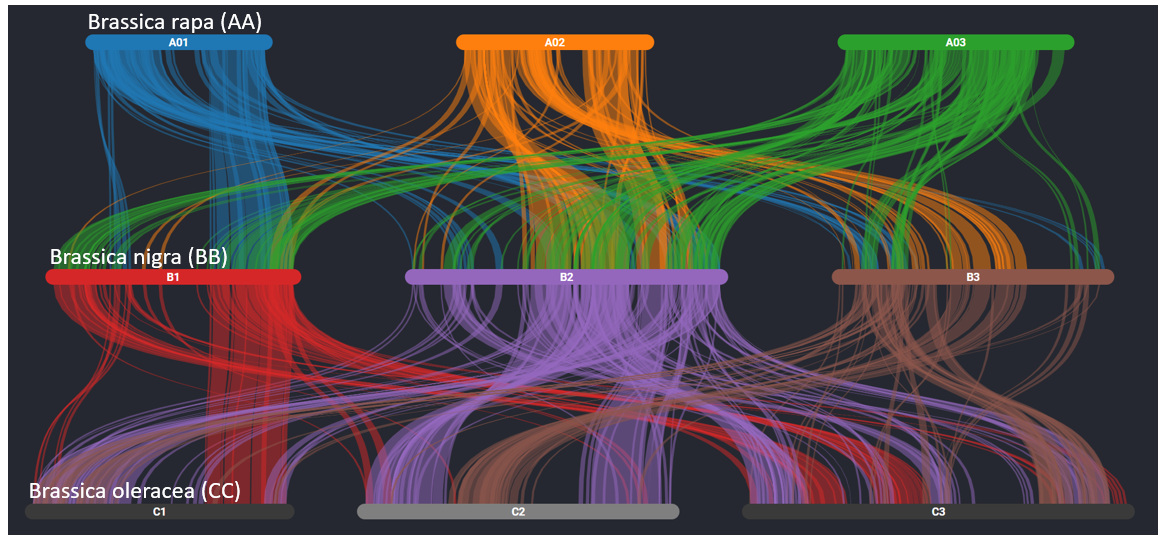
\includegraphics[width=1\linewidth]{images/ch_5_tree_plot.PNG}
  \captionof{figure}{Tree plot showing multi level synteny between the three ancestral genomes from \textit{Brassica} genus.} 
  \label{fig:ch_5_tree_plot}
\end{figure} 

\textit{Tree Plot:} This plot is simply an extension of the primary 2 axis parallel plot that is used in the single analysis mode. Users are first given the option to select the number of layers they need, and then, they are required to choose the chromosomes they need in every layer individually. Chromosomes are then stacked in multiple layers vertically and conserved regions in the chromosomes in every layer are linked bidirectionally. Starting from the top layer every chromosome acts as a parent node and is linked to all the chromosomes directly below it if conservation exists, thus forming a tree-like pattern that can be used to look for conserved regions in ancestral species, as shown in Figure \ref{fig:ch_5_tree_plot}, where synteny between the first three chromosomes is shown for three ancestral genomes of \textit{Brassica} genus from the \textbf{Triangle of U} evolutionary theory\cite{cheng2014genome}. Users are further given the option to filter through the conserved regions by clicking on a chromosome to visualize just the conserved blocks emerging from it at every layer. A dual filter toggle is also provided which when turned on ensures that chromosomal filtering occurs bidirectionally meaning conserved links that both emerge from a chromosome into the the layer below and the conserved links that join into it from the layer above it are both filtered.

\begin{figure}
  \centering
  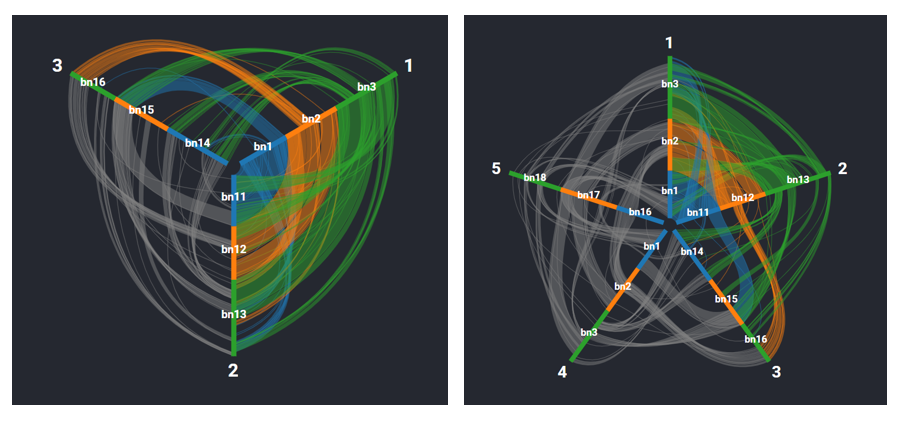
\includegraphics[width=1\linewidth]{images/ch_5_hive_plot.PNG}
  \captionof{figure}{Hive plots showing 3 way synteny(left) and 5 way synteny(right) in \textit{Brassica napus} respectively.} 
  \label{fig:ch_5_hive_plot}
\end{figure} 


\textit{Hive Plot:} These plots have recently gained a lot of traction in large scale network visualizations such as gene regulatory networks due to the high degree of perceptual uniformity that they offer\cite{krzywinski2011hive}. They have also been demonstrated as good alternatives for Circos \cite{krzywinski2009circos} style plots in representing three-way genome alignments. Hive plots are based on a network layout where nodes are placed in radially oriented axes with a linear scale, and edges are drawn between the nodes to encode additional information. In our case, the nodes represent chromosomes, and they are ordered sequentially based on the order in which they are present in the genome. The radial angles between the axes are chosen based on the number of axes present to ensure uniformity. Conserved regions between the chromosomes are then linked through connecting ribbons which are drawn using \textit{Bezier} curves to reduce visual clutter and are bundled together. Unlike the pairwise comparison scenarios, hive plots do not have a single source axis as all axes are uniform in a multi way comparison scenario. So connected ribbons are not coloured to represent the chromosomes they emerge from and are instead left to be translucent gray. User interactions with the hive plot are used to select the source axis. When a user clicks on a particular radial axis, all the connected ribbons emerging from it are coloured based on the chromosomes they belong to in that particular axis. This form of variable encoding based on user choice can be useful in selectively identifying patterns for every genome represented in one radial axis. To use the hive plot users are first required to select the number of radial axes they need and are then required to select the chromosomes to be encoded in each axes. The generated hive chart can then be annotated with chromosomal labels that are hidden by default but can be toggled on/off using a checkbox present in the filter panel. The scales for the radial axes are calculated based on the genomic size of all the chromosomes included in the chart. This ensures that chromosomes that are small in terms of the number of base pairs they contain show up as smaller edges. This can further mean that the sizes of the radial axes of the hive chart can vary depending on the chromosomes that are represented in them. Our interface also provides a \textit{Normalized length} checkbox that can be toggled \textbf{ON} to make the hive chart perfectly uniform. This is achieved by using a variable linear scale for every axis while keeping its total length constant.

\section{Usability Features}
As SynVisio developed into a full-scale application, we were provided with several non-functional requirements from our research collaborators. For each of these requirements, we added features that do not change existing visual encoding used in the system but rather enhance overall user experience with the system. 

\subsection{Track Annotation}
The ability to annotate visualizations with additional data in the form of tracks is a feature that is available in most common genome browsers such as JBrowse, GBrowse, and UCSC Genome Browser\cite{skinner2009jbrowse,donlin2009using,karolchik2003ucsc}. However, it has not seen widespread adoption in the existing synteny analysis tools except for Mizbee,  AccuSyn, and GSV\cite{Meyer2009,accusyn,revanna2012web}.  Having tracks annotate existing visualization generated by SynVisio can help researchers in having a better context of the data under investigation as tracks such as gene counts and SNP(single nucleotide polymorphisms) variations can highlight regions of interest in the entire genome. In our system users can upload a track along with their initial data file in a BedGraph file format which is a standard format used in representing continuous-valued data as tracks. Our system parses the data in the track file and automatically groups it based on the chromosomal widths into distinct regions for each chromosome so that the data can be loaded on demand when users select a particular set of chromosomes for their visualization. We also calculate the maximum and minimum values in the file and use them to generate a linear scale. We limit the number of tracks that a user can annotate a chart with to prevent overcrowding in the visual representation.

\begin{figure}
  \centering
  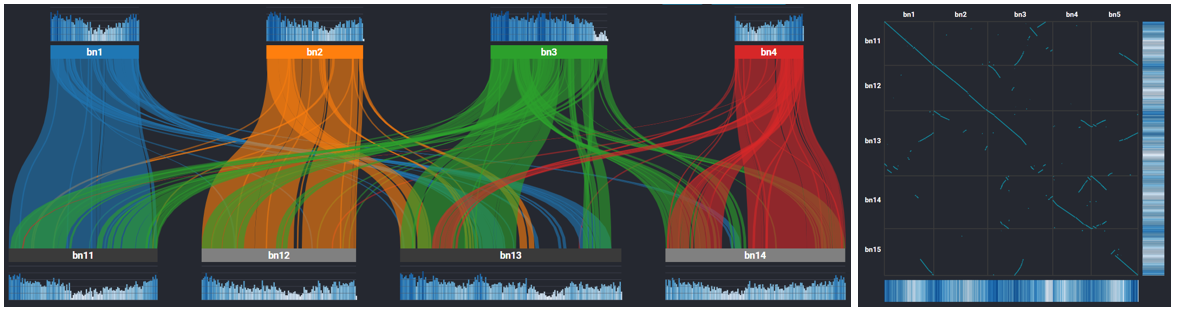
\includegraphics[width=1\linewidth]{images/ch_5_tracks.PNG}
  \captionof{figure}{Additional tracks showing gene count as a histogram in the Parallel plot (left) and as a heat-map in the Dot plot (right).}
  \label{fig:ch_5_tracks}
\end{figure}
When SynVisio detects additional track data in the system, it automatically provides a new button next to the chromosome selection panel called \textit{Toggle Tracks}, which controls
the visibility of tracks in our interface. We offer four types of tracks: heatmap, histogram, linechart and a scatter plot. The heatmap uses a sequential color scale to encode the values in increasing order from white to dark blue. The same color scale is also used for the histogram and the scatter plot along with their default encoding scheme. The linechart alone doesn't use any color encoding and is represented in a single base colour. All the vertical positions in the charts are rendered using the previously calculated linear scale which is also used to generate five equidistant vertical grid lines for the tracks. For the parallel plot, the tracks are added on the outer side of the visualization with one track sitting above the source genome and the other track sitting below the target genome. Since the tracks are accurately mapped to the chromosomes, the pill shaped design of the chromosome is replaced with rectangles to ensure the start and the end of the chromosomes are consistent with the start and the end of the tracks. For the dot plot the tracks are annotated along the \textit{x,y} axes on the opposite side of the chromosome labels.


\subsection{Gene Search Panel}
SynVisio maintains an in-memory collection of all the genes present in a genome or a pair of genomes under investigation in the interface. This can be used to quickly lookup conserved regions that contain a particular gene of interest. This feature is presented in the \textit{Gene Search Panel} situated at the top of the dashboard. Users can key in a \textit{Gene ID} and click on the search button. The system then checks on the collection of genes and presents all matching alignments containing that particular gene as clickable buttons along with information on the source and target chromosomes of the alignment and its orientation. Clicking on any alignment launches the Chromosome Mode of SynVisio between the pair of Chromosomes that contain the alignment block, and the alignment block itself is highlighted in a pale white colour, as shown in figure \ref{fig:ch_5_gene_serach}. 

\begin{figure}
  \centering
  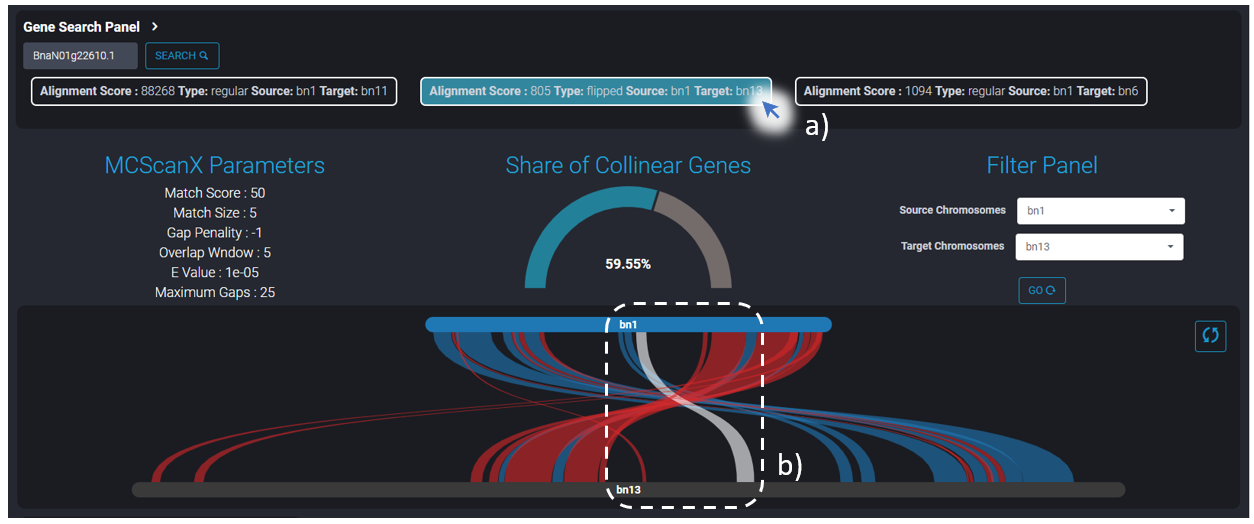
\includegraphics[width=1\linewidth]{images/ch_5_gene_serach.PNG}
  \captionof{figure}{Gene Search Panel in SynVisio, with matching alignments present as clickable buttons (a) that when clicked highlight the corresponding alignment (b).}
  \label{fig:ch_5_gene_serach}
\end{figure}


\subsection{Support to Map Unplaced Scaffolds}
Genome assembly is the process in which a genome is pieced together into a large number of contigs computationally from randomly sequenced reads (DNA/RNA segments)\cite{hunt2014comprehensive}. These contigs are then assembled into longer scaffolds which are in turn further assembled into chromosomes. However, due to lack of sufficient mapping information the position and orientation of certain scaffolds remains unknown and also many genome assemblies only assemble data to the scaffold level \cite{ensembl}. This makes it impossible visualize synteny as most synteny tools only offer mapping based on chromosomal order. SynVisio attempts to solve this problem by letting users visualize the synteny between unplaced or unlocalised scaffolds. By default SynVisio ignores Scaffolds regions as there can be quite a lot of them cluttering the visualization, however users can opt out of ignoring scaffolds. This will give users a list of scaffolds to select in the source and target chromosome list in the filter panel at the top of the dashboard. This feature is particularly important to users who would like to visualize collinearity between unplaced scaffolds and known sequenced genomes to improve their genome assembly results. 


\subsection{Image Export}
Most synteny browsers such as MultiSyn, Synteny Portal, and GSV\cite{baek2016multisyn,lee2016syntenyportal,revanna2011gsv} have the option to export images except for Mizbee\cite{Meyer2009} which is designed more for analysis than image generation.
SynVisio, however, can work both as an analysis tool and can also generate high-quality publication ready images when required. SynVisio renders visualizations on screen in the transform and scale-invariant vector graphics format, and these can be downloaded using the export toggle provided as a floating button situated in the bottom corner of the screen. Furthermore, SynVisio exports visualizations along with the updates made to them by users as they interact with them in real-time. So changes such as adding tracks, filtering out low similarity score blocks and highlighting a particular chromosome are all retained in the exported image. A final advantage of exporting images in SVG format is that these images can be edited and the colours of the individual elements changed using vector graphic editors like \textbf{Inkscape} and \textbf{Adobe Illustrator}.

\subsection{Revisitation Support}
Multi-scale visualization systems are effective at exploring large datasets as they help researchers in following the visual information seeking mantra of \textit{overview first, zoom and filter followed by details on demand}\cite{Shneiderman96theeyes}. They achieve this by changing the visual representation of the data at different levels of abstraction as the user zooms in for closer inspection\cite{Stolte}. This however can cause the user to lose context of their position in a particular graph as they constantly need to switch between different kinds of visual representations.
Although humans are good at leveraging spatial cognition to remember locations of objects in information workspace tasks\cite{datamountain} context switching visual systems can disrupt this ability. To fix this issue, SynVisio lets users keep track of their actions through a visual snapshot store feature. It follows the functioning of a traditional information retrieval system by preserving the sequence of actions that lead to the current state of the visual interface in a snapshot. Users can then store this snapshot by clicking on the floating camera button at the bottom left corner of the interface. Snapshots are stored sequentially and are available for revisitation at the \textit{Snapshot Store Panel} situated at the top of the interface. Clicking on any snapshot in the panel automatically recreates the stored visual state of the system. The snapshots, however, are stored only as an in-memory collection in the system and so do not persist over page reloads or when users switch the input data files.


\section{System Architecture}

The internet has had an immense impact on the ability to access information and communicate ideas. Recent trends in software development have shown that there is an exponential increase in the development of internet-based web applications that are built using a mixture of \textbf{HTML5}, \textbf{JavaScript} and \textbf{CSS3} compared to native applications.
This is due to the ease of availability of web applications and their device agnostic design that can ensure that they run independently of the operating system or the device type. Although some synteny browsers have been developed as native applications like Mizbee and SyMAP\cite{Meyer2009,soderlund2011symap}, most of the latest synteny browsers like MultiSyn, mGSV and Synteny Portal\cite{baek2016multisyn,revanna2011gsv,lee2016syntenyportal} all adopt a web-based approach. Following this trend, we developed SynVisio as a web-based application that can be accessed for free through the internet at \url{https://synvisio.usask.ca}.

There are two main design patterns for web applications: Single-page application and Multi-page application. The choice of the design patterns is based on the content being served. Single-page applications request the content markup and the data independently and render pages dynamically in the browser through JavaScript. This makes them fast and responsive despite the initial delay in loading all content in a single bundle during page load. There are no subsequent page reloads however and all further requests are purely for data which has a significantly smaller payload. Multi-page applications, on the other hand, follow a more traditional approach with changes and interactions being sent to the server, which responds back with a new page to be rendered by the browser. This constant back and forth between the browser and the server can make these systems cumbersome to use due to the continuous delay. However Multi-page applications are more secure compared to Single-page applications which can be susceptible to Cross-Site Scripting (XSS) attacks.
Although users aren't concerned with software architecture, as they focus on tasks and not the structure of a system, it can be a determinant for the usability of any system. Proper information architecture should offer users logical structures that can aid them in navigating towards the right answers and completing the required tasks\cite{rosenfeld2002information}. Thus for SynVisio, we adopt the Single-page architecture design and render visualizations in the browser instead of having them shipped from a remote server as this allows for users to interact with them in real-time and offers a smooth genome browsing experience\cite{nielsen2010visualizing}. 

This form of a thick client architecture model where data processing is managed locally in the client machine also ensures that all the data files that researchers upload to our website remain secure within the same machine and are not sent to any other remote server. However, processing data files in the web browser comes with its own set of complications as JavaScript has a single threaded environment and any intensive data processing can block the main thread limiting user interactivity in the page. To address this issue we use the \textbf{Web Workers API} to spawn background scripts that can handle computationally intensive tasks without blocking the main user interface\cite{webworkers}. Every user uploaded file is processed in an independent thread through a web worker and the processed results are then combined to form an in-memory dictionary of all the genomic links, classified based on the chromosomes present in the genome. This dictionary is then used every time a user selects a pair of chromosomes to query the required set of genomic links to be visualized.

The base user interface of SynVisio is built using two JavaScript libraries React.JS\cite{react} to handle user interactions and render content and D3.JS\cite{d3js} to generate visualizations.
React is a popular JavaScript library maintained by Facebook\cite{facebook} that is used in building user interfaces in Single-page applications. It can efficiently manipulate the representation of a web-page which is called the document object model(DOM). It does this through a process of reconciliation with an in-memory representation of the actual DOM called the virtual DOM. This is particularly useful in our scenario as all visualizations are rendered through vector graphics and so are part of the actual DOM structure.Thus as the size of the data being visualized increases there is a corresponding increase in the number of visual elements in the DOM. However by using React we can handle large DOM networks efficiently by deferring updates only when necessary. The second major advantage to using react is that it follows a component-based model where every part of the interface is built using a set of reusable components that render differently based on the data being passed to them. This enables us to rapidly switch the generated visualizations on the screen by simply modifying the underlying data provided to the component. This is particularly useful in implementing interactive real-time filtering as any filtering done to the underlying dataset is reflect onto the actual visualization. This feature is also used in providing support for the revisitation feature discussed in section 5.3.4 where every saved stamp is essentially a data object that is stored and passed onto the graphical component to recreate the required visualization.

All visualizations in SynVisio are rendered as simple vector graphics(SVG) with the path values of the underlying graphical elements being calculated using D3.JS. These include the mathematical calculation involved in the interpolation of points that connect conserved regions and scale transformations from genomic distances to pixels. Finally, SynVisio can switch to rendering in canvas instead of vector graphics when there are more than 20,000 graphical elements in a visualization, as SVG performance can be hindered at higher numbers. This also limits the user interactions that are possible with the visualization, and a warning message is shown to the user to select a smaller subset of the dataset or an alternate representation with fewer visual elements. This adaptive mode of SynVisio was built to ensure that even extremely large datasets can be viewed in the system without a breakdown in the system performance.

